The search for hints of supersymmetric particles is among the important goals of the LHC physics program. As discussed in Sec.~\ref{subsec:susy_collider}, searches performed at $\sqrt{s} = 7$\tev have constrained the allowed parameter space for light-flavour squarks and gluinos already up to around 800\gev and 1\tev for light LSP masses, respectively. However, the increased centre of mass energy from 7\tev to 8\tev and the recorded dataset which is around four times larger than at 7\tev provide the opportunity to extend the reach of such searches into entirely unexplored parameter regions. In Fig.~\ref{fig:susy_theory_xs} the theory cross section for the production of supersymmetric particles is shown as function of the SUSY particle mass. The y-axis on the right indicates how many events are expected in 20\fbinv of pp collision data at the LHC at $\sqrt{s}=8$\tev. \\

\begin{figure}[!h]
  \centering
  \begin{tabular}{c}
                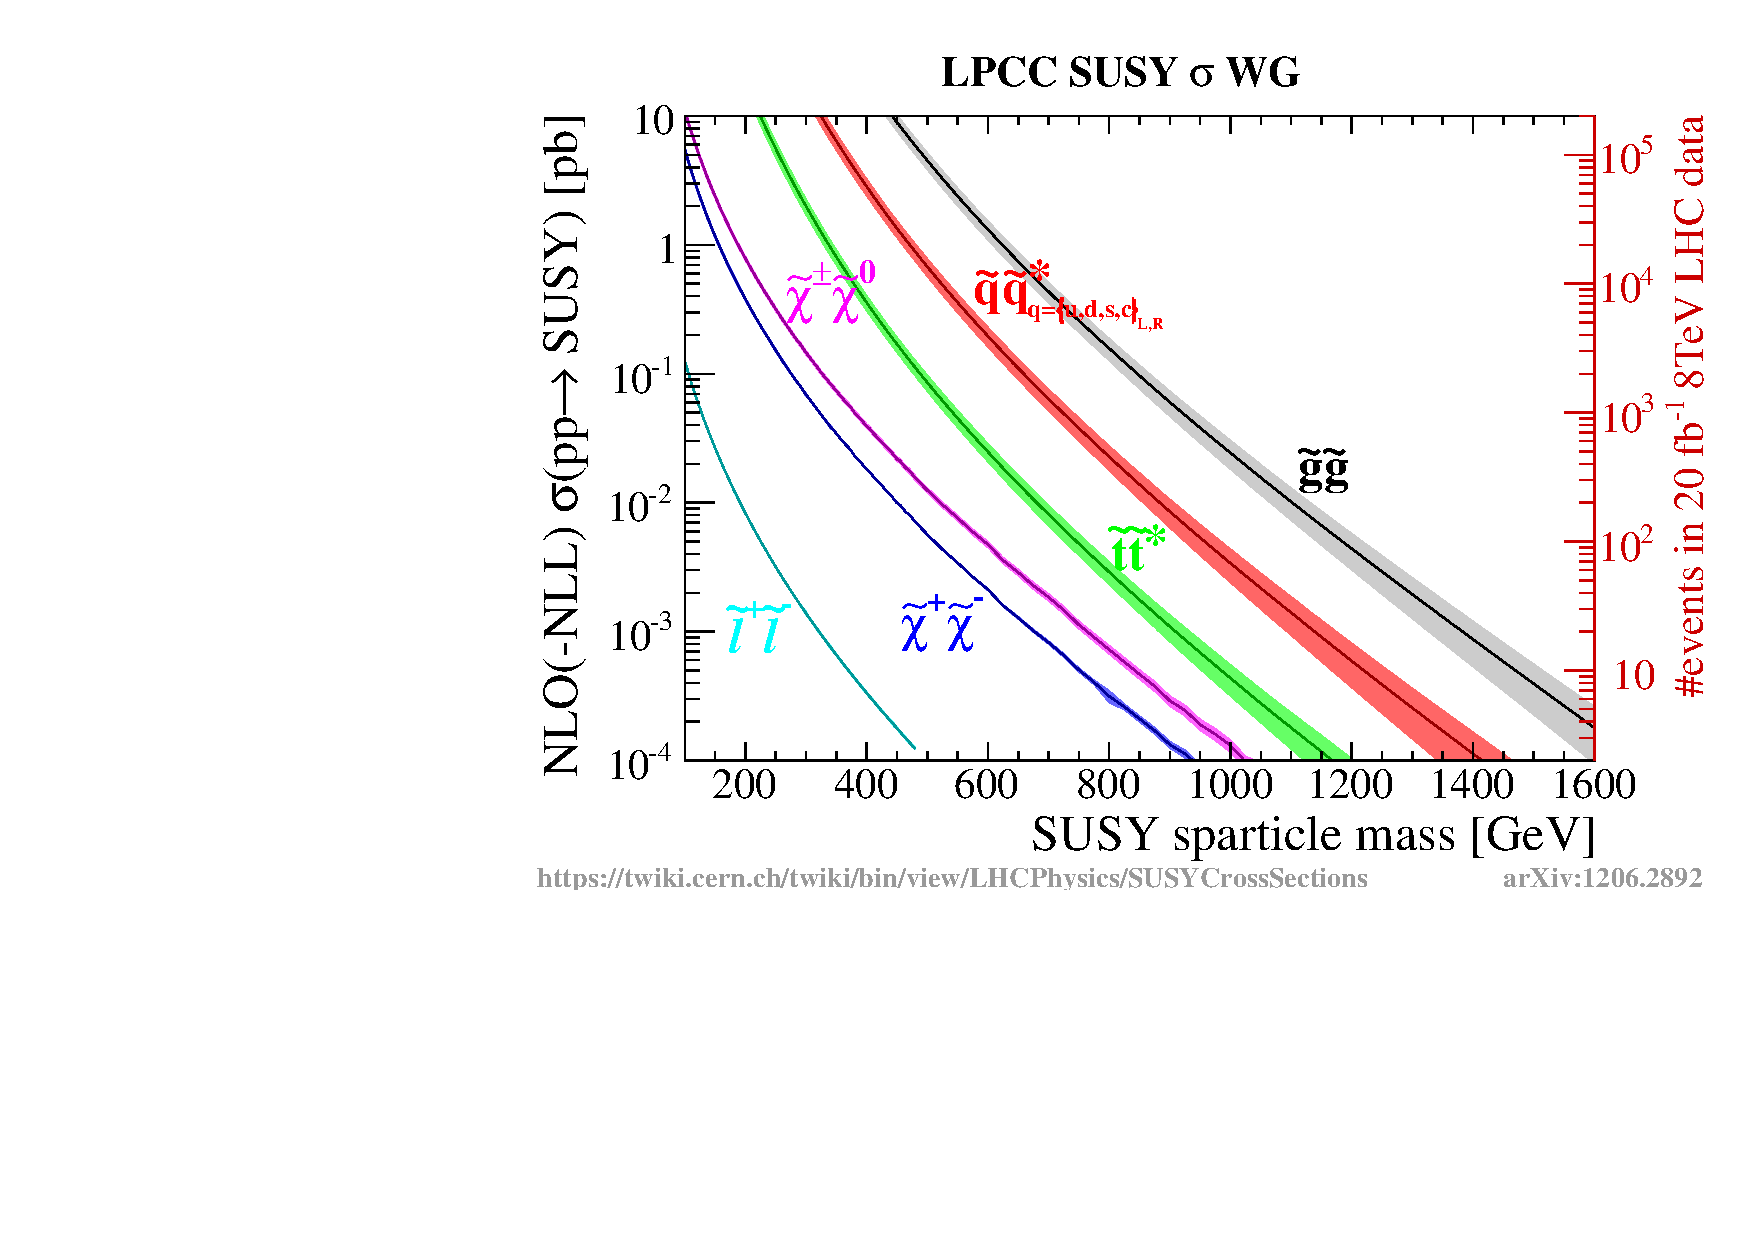
\includegraphics[width=0.65\textwidth]{figures/xsections_strong.pdf} 
  \end{tabular}
  \caption{Theory cross sections for selected SUSY processes as function of the SUSY sparticle mass. The y-axis on the right indicates the expected number of events in 20\fbinv of pp collision data at the LHC at $\sqrt{s}=8$\tev. Taken from~\cite{Kramer:2012bx}.}
  \label{fig:susy_theory_xs}
\end{figure}
It is visible that especially light-squarks and gluinos are expected at a sizable rate even for high masses above 1\tev. For instance, around 100 pairs of gluinos are expected at a mass of 1200\gev. \\
The analysis presented in this Chapter is aiming at a search for supersymmetric cascade decays arising from strongly produced light-flavour squarks or gluinos. Thus, events are selected based on the scalar sum of the jet transverse momenta (\HT), the missing transverse momentum calculated from the jet momenta (\MHT) and the number of jets (\NJets). However, the generic structure makes the analysis in principle sensitive to any new physics model that manifests in final states containing several hard jets accompanied by missing transverse energy. \\
After the description of the event selection (Sec.~\ref{sec:RA2_sel}), it is discussed how contributions from standard model processes to the selected final state are estimated. Special emphasis is put on the estimation of the QCD multijet background (Sec.~\ref{subsec:RA2_QCD}). Finally, results are presented and interpreted in various simplified supersymmetric models (Sec.~\ref{sec:RA2_results}). Parts of this Chapter are taken from~\cite{bib:AN-12-350}, having been written by the author. The analysis is published in~\cite{Chatrchyan:2014lfa}.    
\section{Event Selection}
\label{sec:RA2_sel}

\subsection{Data Samples and Trigger}
\label{subsec:RA2_samples_trigger}
The analysis is based on pp collision data recorded with the CMS detector at a centre-of-mass energy of $\sqrt{s} = 8$\tev. This corresponds to an integrated luminosity of 19.5\fbinv for all sub-detectors fully functional. \\
The data have been collected by triggering on \HT, the scalar sum of the jet transverse momenta, and \met, the missing transverse energy. An overview of the considered runs and the integrated luminosity is shown together with the respective HLT trigger paths in Tab.~\ref{tab:RA2_trigger}. \HT and \met are calculated from particle-flow objects at trigger level with nominal thresholds of 350\gev and 100\gev, respectively. Jets considered in this calculation are reconstructed with the anti-$k_T$ algorithm and distance parameter $R = 0.5$. The labelling \textit{PFNoPU} indicates that for that particular runs also charged-hadron subtraction was applied to jets at trigger level. \\
\begin{table}[!b]
\centering
\caption{Utilized signal trigger paths in individual run ranges listed together with the integrated luminosity.}
\label{tab:RA2_trigger}
 \makebox[\linewidth]{
\begin{tabular}{lccc}
\multicolumn{4}{c}{} \\
\toprule
 Trigger path & Run range & Luminosity [\fbinv] \\
\midrule
 HLT\_PFHT350\_PFMET100 & 190456 -- 196531 & 0.9 \\
 & & & \\
 HLT\_PFHT350\_PFMET100 & 190782 -- 190949 & 4.4 \\
 & & & \\
 HLT\_PFNoPUHT350\_PFMET100 & 198022 -- 198523 & 6.9 \\
 & & & \\
 HLT\_PFNoPUHT350\_PFMET100 & 198524 -- 208686 & 7.3 \\
\bottomrule
\end{tabular}}
\end{table}  
In order to determine the offline values for \HT and \MHT (calculated according to the definition following in Sec.~\ref{subsec:RA2_baseline}) for which the triggers reach the plateau efficiency, the trigger efficiencies are measured with respect to a single electron trigger (HLT\_Ele27\_WP80). In principal, an orthogonal trigger is needed in order to get an unbiased estimate of the trigger efficiency. However, due to the PF-algorithm all subdetectors are used simultaneously to reconstruct the particles in an event. Hence, no independent trigger paths providing enough statistical precision are available. Consequently, only the reach of a plateau efficiency for a certain trigger path can be determined while the absolute efficiency is not accessible. The determination of the trigger plateau efficiency is performed for different jet multiplicity intervals (\NJets~$ = 3-5$, \NJets~$ = 6-7$ and \NJets~$ \ge 8$). The obtained trigger turn-on curves for the two different HLT paths are shown as function of offline \HT and \MHT for jet multiplicity \NJets~$ = 3-5$ in Fig.~\ref{fig:trig_eff_3njets5}. For both trigger paths, the efficiency plateau is reached around offline values of \HT$ = 500$\gev and \MHT$ = 200$\gev. The integrated trigger efficiencies for these particular values in different jet multiplicity intervals are summarized with statistical uncertainties in Tab.~\ref{tab:trig_eff}. In general, they are close to 100\% with small uncertainties below 1\%. However, for the highest jet multiplicity selection of \NJets~$ \ge 8$ only few events where selected such that statistical uncertainties are few 10\% large. Though, no hints for a systematic inefficiency have been observed and the signal triggers are considered as fully efficient with an uncertainty of $1\%$ for offline values of \HT$ > 500$\gev and \MHT$ > 200$\gev independent of the jet multiplicity. 

\begin{figure}[!t]
  \centering
  \begin{tabular}{cc}
                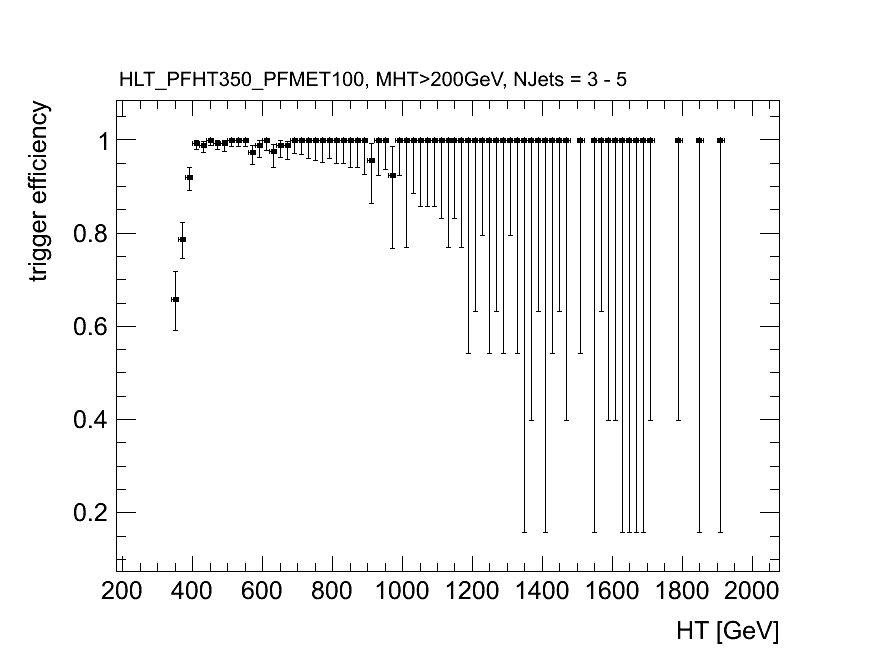
\includegraphics[width=0.49\textwidth]{figures/turn_on_HT_TagEle27WP80_ProbePFHT350PFMET100_MHT200_chs_NJets3_5.png} &
                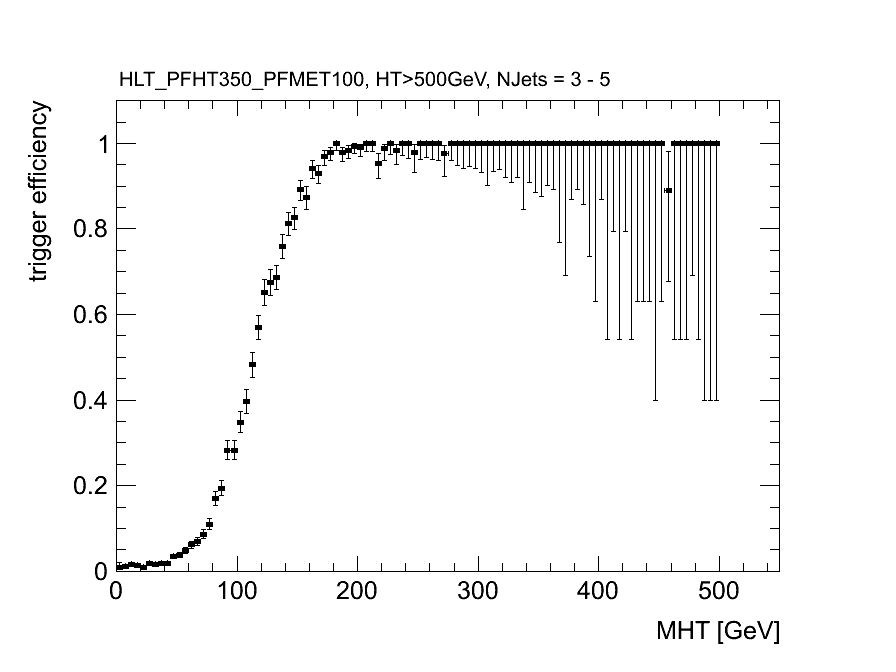
\includegraphics[width=0.49\textwidth]{figures/turn_on_MHT_TagEle27WP80_ProbePFHT350PFMET100_HT500_chs_NJets3_5.png} \\
                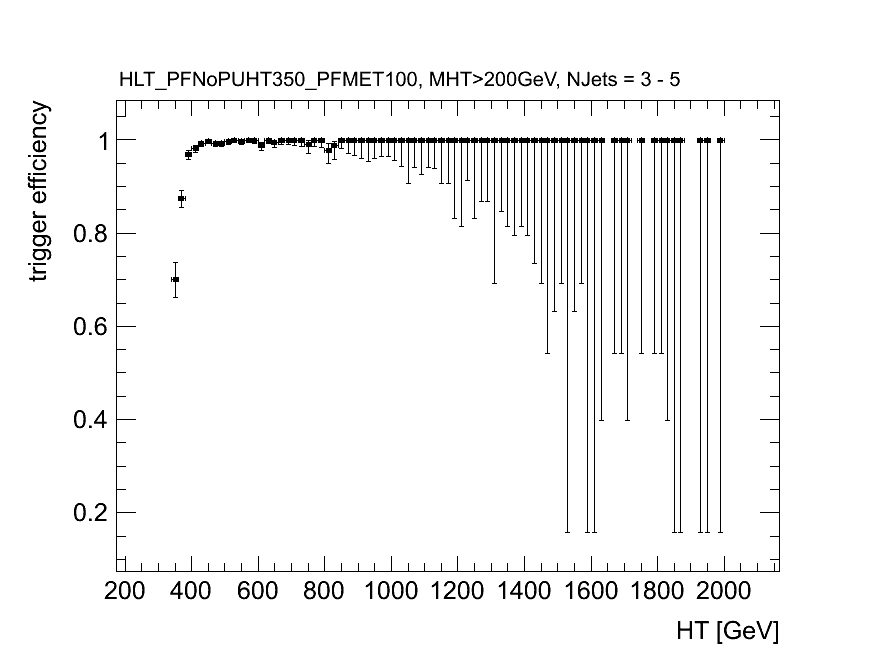
\includegraphics[width=0.49\textwidth]{figures/turn_on_HT_TagEle27WP80_ProbePFNoPUHT350PFMET100_MHT200_chs_NJets3_5.png} &
                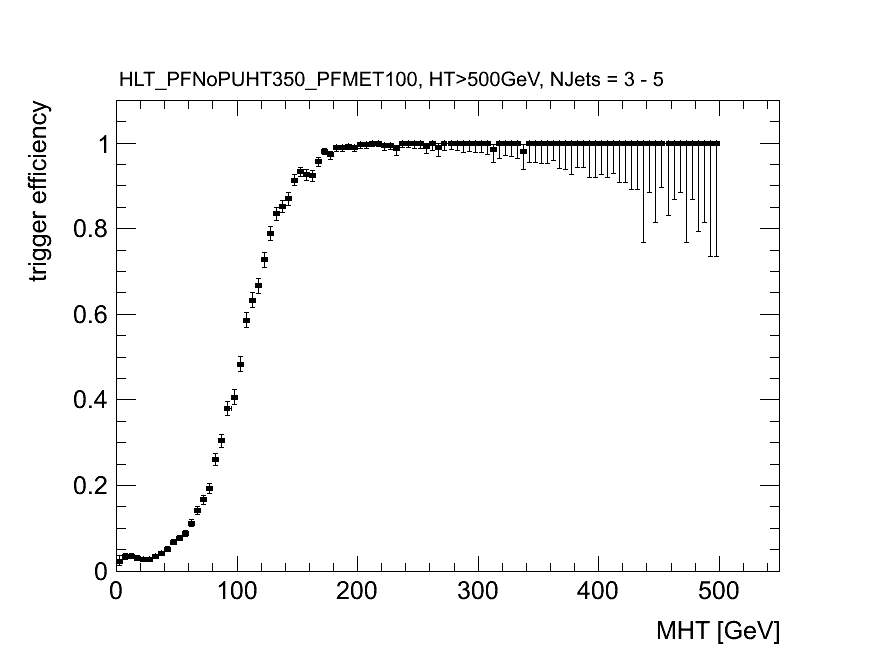
\includegraphics[width=0.49\textwidth]{figures/turn_on_MHT_TagEle27WP80_ProbePFNoPUHT350PFMET100_HT500_chs_NJets3_5.png} \\
  \end{tabular}
\caption{Measured trigger efficiency for paths HLT\_PFHT350\_PFMET100 (\textit{top}) and HLT\_PFNoPUHT350\_PFMET100 (\textit{bottom}) as a function of \HT (\textit{left}) and \MHT (\textit{right}) shown for $3 \leq$ \NJets $\leq 5$.} 
  \label{fig:trig_eff_3njets5}
\end{figure}

\begin{table}[!t]
  \caption{Summary of total trigger efficiencies of the signal triggers for selections of offline \HT$ > 500$\gev and \MHT$ > 200$\gev in different jet multiplicity intervals.} 
  \label{tab:trig_eff}
  \begin{center}
    \begin{tabular}{lcc}
      \toprule
      \NJets & HLT\_PFHT350\_PFMET100 &  HLT\_PFNoPUHT350\_PFMET100\\
      \midrule
      3 - 5   & $99.4 _{-0.3} ^{+0.2}$   & $99.8 _{-0.1} ^{+0.1}$\\
      6 - 7   & $99.1 _{-2.0} ^{+0.7}$   & $100.0 _{-0.6} ^{+0.0}$\\
      $\ge$ 8 & $100.0 _{-36.9} ^{+0.0}$ & $100.0 _{-10.9} ^{+0.0}$\\
      \bottomrule
    \end{tabular}
  \end{center}
\end{table}

\subsection{Event Cleaning}
\label{subsec:RA2_cleaning}
The analysis presented in this Chapter heavily realies on a precise measurement of the momentum imbalance in the event. In order to remove events with large values of fake missing momentum arising from detector noise a dedicated sequence of cleaning filters is applied. 
\begin{description}
 \item{\textbf{Primary Vertex and Beam Halo:}} Only events with at least one high-quality primary vertex are considered in the analysis. A primary vertex is classified as good, if it has more than four associated tracks and is located within 24\,cm in $z$ and 2\,cm in $xy$ direction from the nominal interaction point (\textit{good-vertex filter}). In order to reject events in which protons from the beam interact with residual gas molecules in the beam pipe, the CSC subdetector is used to identify muons moving parallel to the beam (\textit{beam-halo filter}).
 \item{\textbf{Anomalous Calorimeter Signals:}} Some events are affected by particles hitting the readout electronics or other technical instrumentation and cause anomalous signals in the ECAL or HCAL. For instance, noise in the readout system can fake artifical energy deposits at random times. Such events are identified based on timing and pulse-shape information (\textit{HBHE noise filter}). Furthermore, two $5 \times 5 $ supercrystal regions in the EE have been observed to give anomalously high energies. They are removed by imposing selections on the deposited energy in the identified supercrystals (\textit{EE bad supercrystal filter}). In order to account for transparency losses in the ECAL crystals, the system is calibrated with a dedicated laser. However, in the data some crystals are observed which receive unphysically large corrections. Events affected by this unusually large ECAL laser correction factors are rejected (\textit{ECAL laser correction filter}). The HCAL is also monitored by a dedicated laser system. Sometimes the laser fires into the collision bunch-crossing resulting in unwanted signals. These events are removed according to an event list indicating the affected events (\textit{HCAL laser filter}). The jet reconstruction utilizes information from the HO. This is used as identifier of significant leakage beyong the HCAl barrel. However, events with anomalous energy deposits in the HO have to be rejected. Thus, events in which the fraction of the momentum deposited in the HO is $> 40\%$ are removed (\textit{HO filter}).
 \item{\textbf{Dead ECAL Cells:}} Some single crystals in the ECAL are affected by malfunctioning. These single dead ECAL cells make up around $1\%$ in total and can be responsible for energy losses resulting in large values of fake-\MHT. Such events can be identified by using the trigger primitive information to determine how much energy was lost (\textit{TP filter}) or by using the surrounding energy of the masked cells (\textit{BE filter}).
 \item{\textbf{Tracking Failure:}} In some events the track reconstruction is observed to fail manifesting in large calorimeter energy deposits with lack of associated tracks. This can be caused e.g. by too many seed clusters or by collisions not taking place in the actual center of the detector. Thus, the scalar sum of track momenta associated to the good vertices divided by \HT in the event has to be larger than 10\% (\textit{tracking failure filter}) and if at least ten tracks are present in the event, good-quality tracks have to be more than 25\% (\textit{beam-scraping filter}). In addition, events with misreconstructed muon momenta in the PF algorithm (\textit{inconsistent muon filter}) or events where soft muons wrongly absorb energy from energetic HCAL towers they traverse (\textit{greedy muon filter}) are rejected. Furthermore, events with coherent noise in the strip tracker can occur. These cause several clusters distributed across the whole detector and lead to the identification of fake tracks. Such events where the track reconstruction aborted can be identified by comparing the number of pixel clusters to the number of strip clusters (\textit{many strip clusters filter}, \textit{too many strip clusters filter}, \textit{log error too many strip clusters filter}). Another failure of track reconstruction occurs sometimes when track seeds from the TOB and TEC are used. Consequently, events are rejected, if a jet with number of charged hadrons above 200 is reconstructed within $0.9 < |\eta| < 1.9$ (\textit{TOB/TEC tracking filter}).
 \item{\textbf{Noise Induced Jets:}} In order to reject events with fake jets from detector noise, events are discarded if the energy of a jet with \pt$ > 30$\gev is composed of more than 95\% from PF photon candidates or more than 90\% from PF neutral hadron energy (\textit{PBNR filter}).
\end{description}

\subsection{Baseline Selection}
\label{subsec:RA2_baseline}
Here comes the baseline selection

\subsection{Exclusive Search Regions}
\label{subsec:RA2_search_regions}

\section{QCD Background Estimation with the Rebalance-And-Smear Method}
\label{subsec:RA2_QCD}

\subsection{Rebalance Procedure using Kinematic Fits}
\label{subsec:RA2_reb}

\subsection{Response Smearing}
\label{subsec:RA2_smear}

\subsection{Validation Tests}
\label{subsec:RA2_clsoure}

\subsection{Systematic Uncertainties}
\label{subsec:RA2_syst_unc}

\subsection{QCD Background Prediction}
\label{subsec:RA2_qcd_pred}

\section{Estimation of Non-QCD Backgrounds}
\label{sec:RA2_Non-QCD}

\subsection{Invisible Z Background}
\label{subsec:RA2_Zinv}

\begin{figure}[!h]
  \centering
\makebox[\linewidth]{
  \begin{tabular}{cc}
                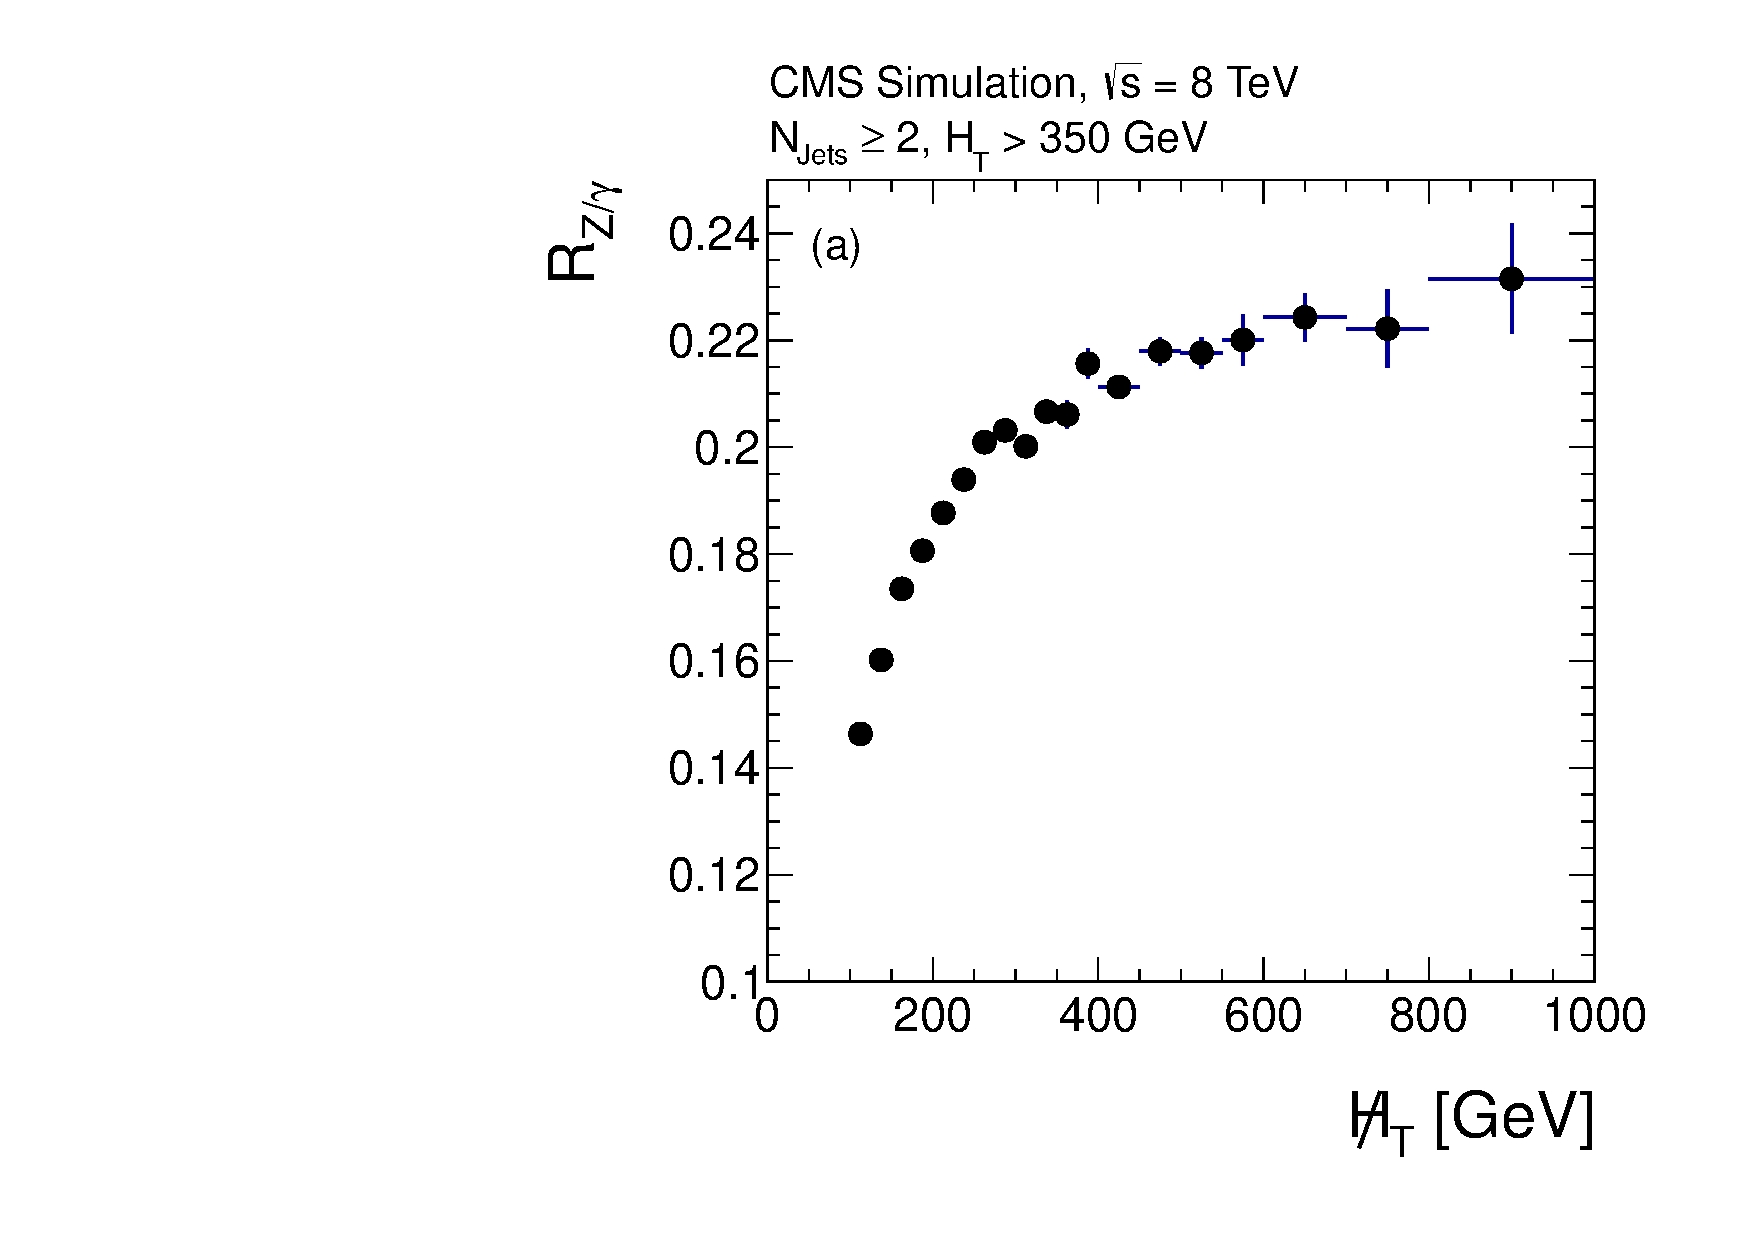
\includegraphics[width=0.4\textwidth]{figures/RA2_Zinv1.pdf} & 
                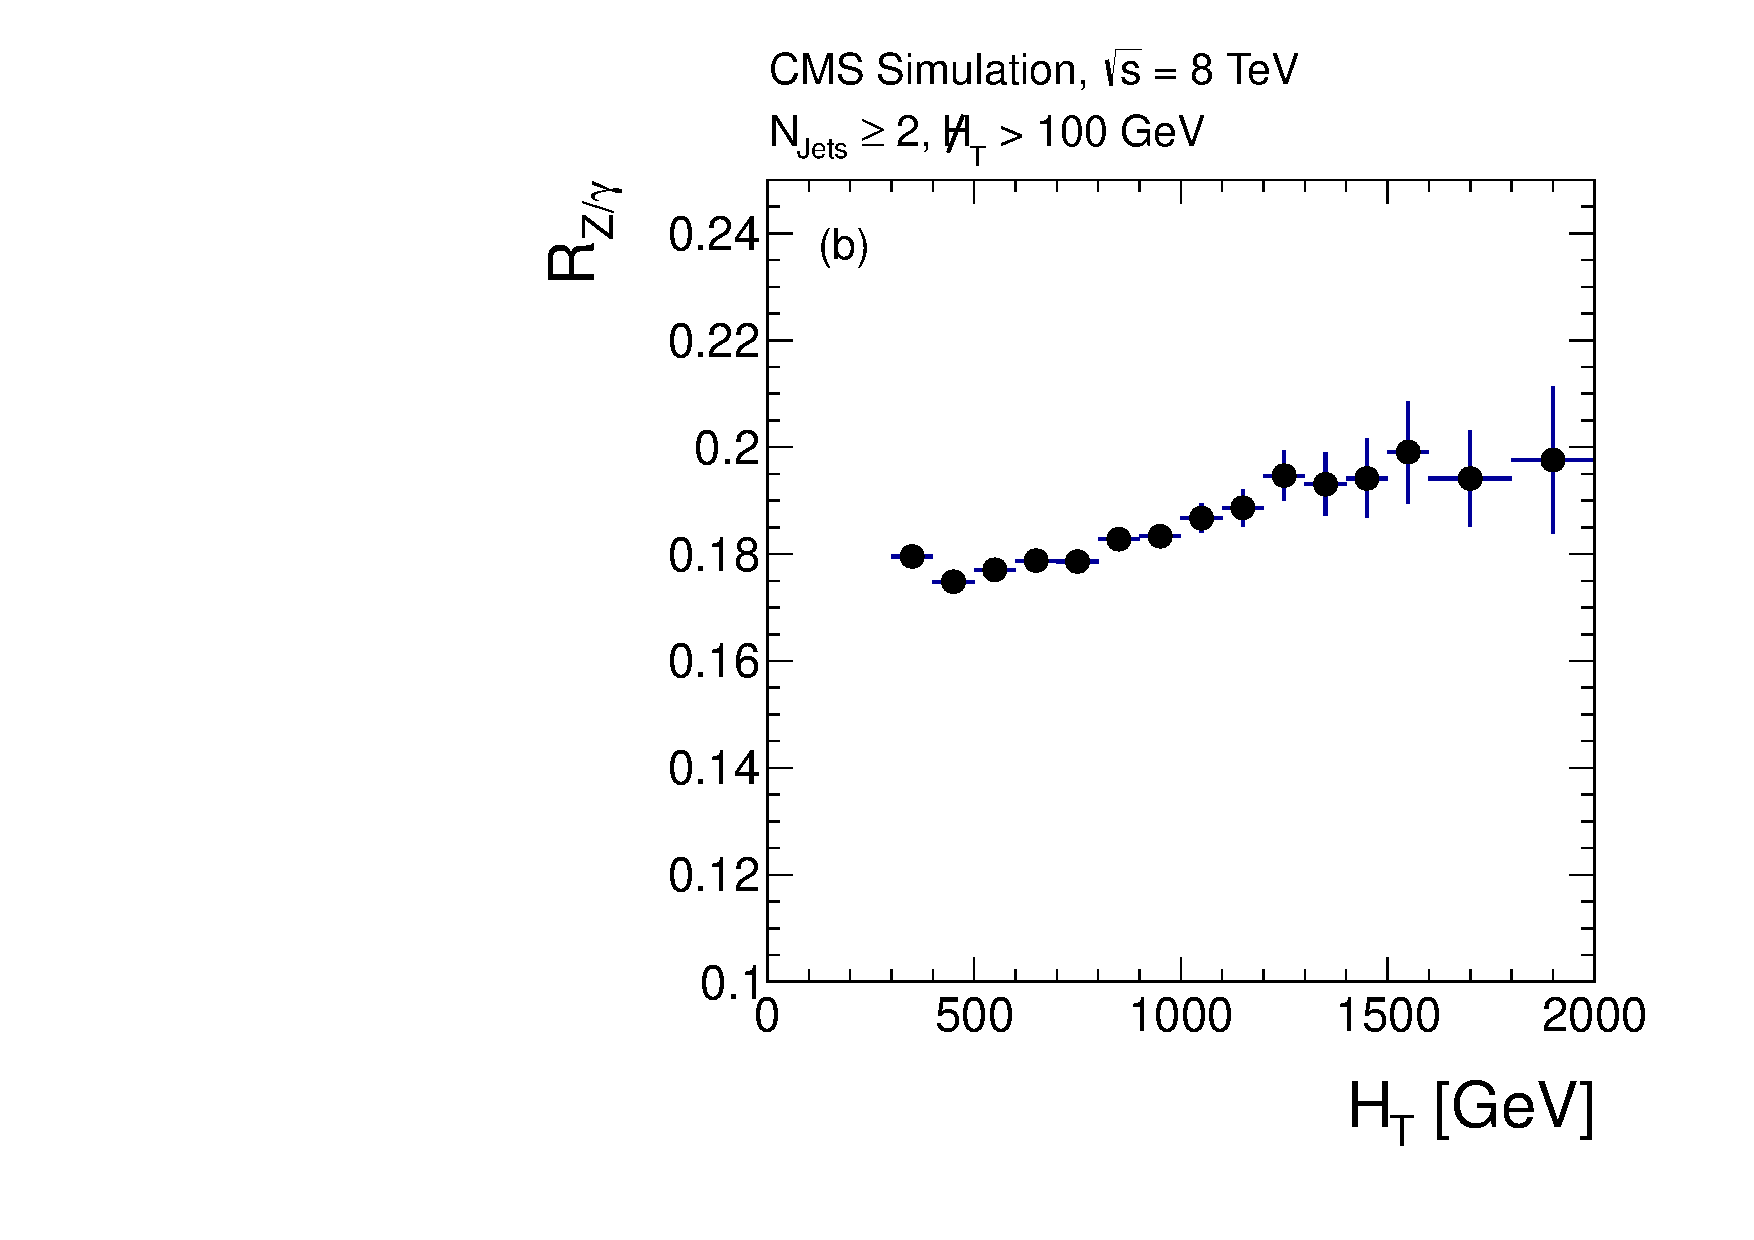
\includegraphics[width=0.4\textwidth]{figures/RA2_Zinv2.pdf} \\
                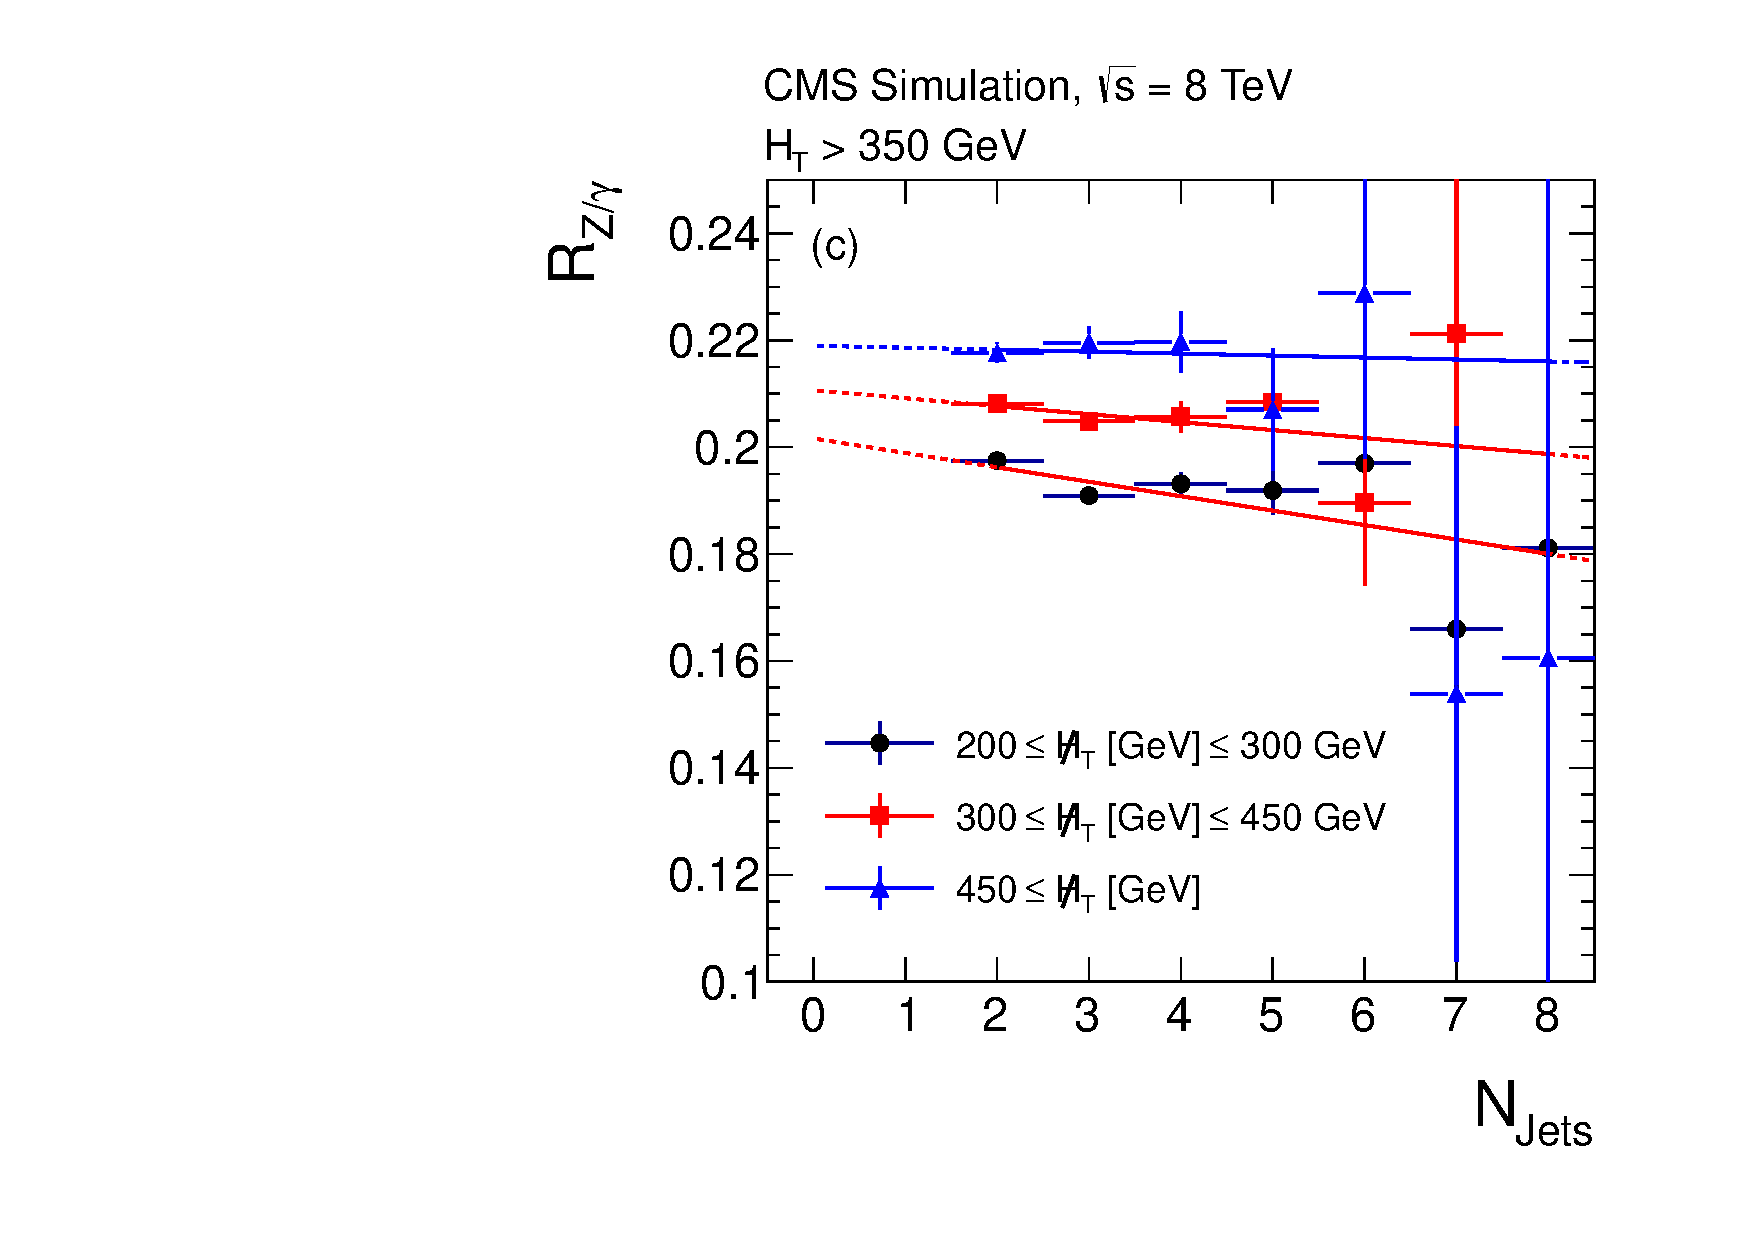
\includegraphics[width=0.4\textwidth]{figures/RA2_Zinv3.pdf} &
                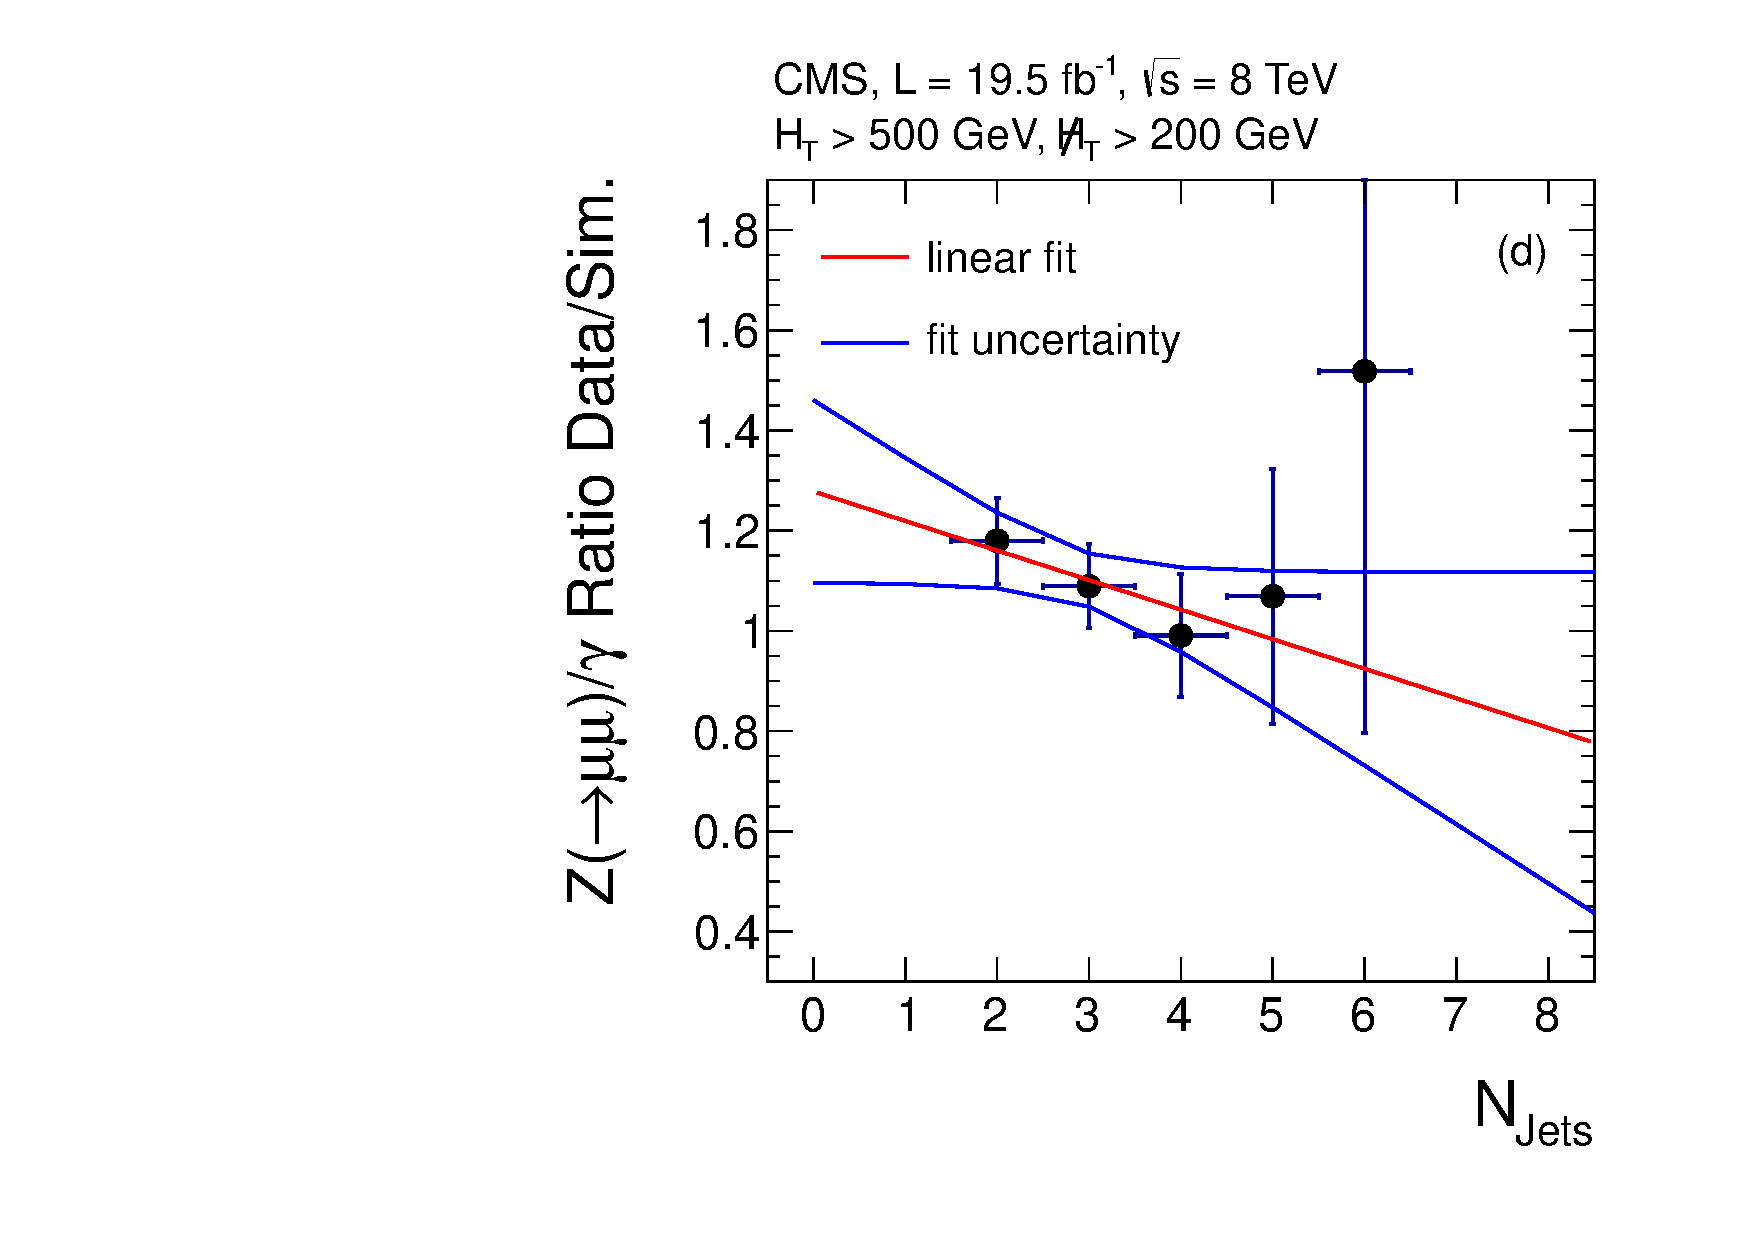
\includegraphics[width=0.4\textwidth]{figures/RA2_Zinv4.pdf}
  \end{tabular}}
  \caption{The simulated ratio $R_{Z/\gamma}$ as a function of (a) MHT, (b) HT, (c) NJets, where the values for three MHT bins are shown with linear fits, and (d) the double ratio of $R_{Z(\mu+\mu-)/\gamma}$, using events from data to those from simulation; the linear fit and its uncertainty band are overlaid. Taken from~\cite{Chatrchyan:2014lfa}.}
  \label{fig:ra2_zinv}
\end{figure}

\subsection{Hadronic $\tau$ Background}
\label{subsec:RA2_tauhad}

\begin{figure}[!h]
  \centering
\makebox[\linewidth]{
  \begin{tabular}{ccc}
                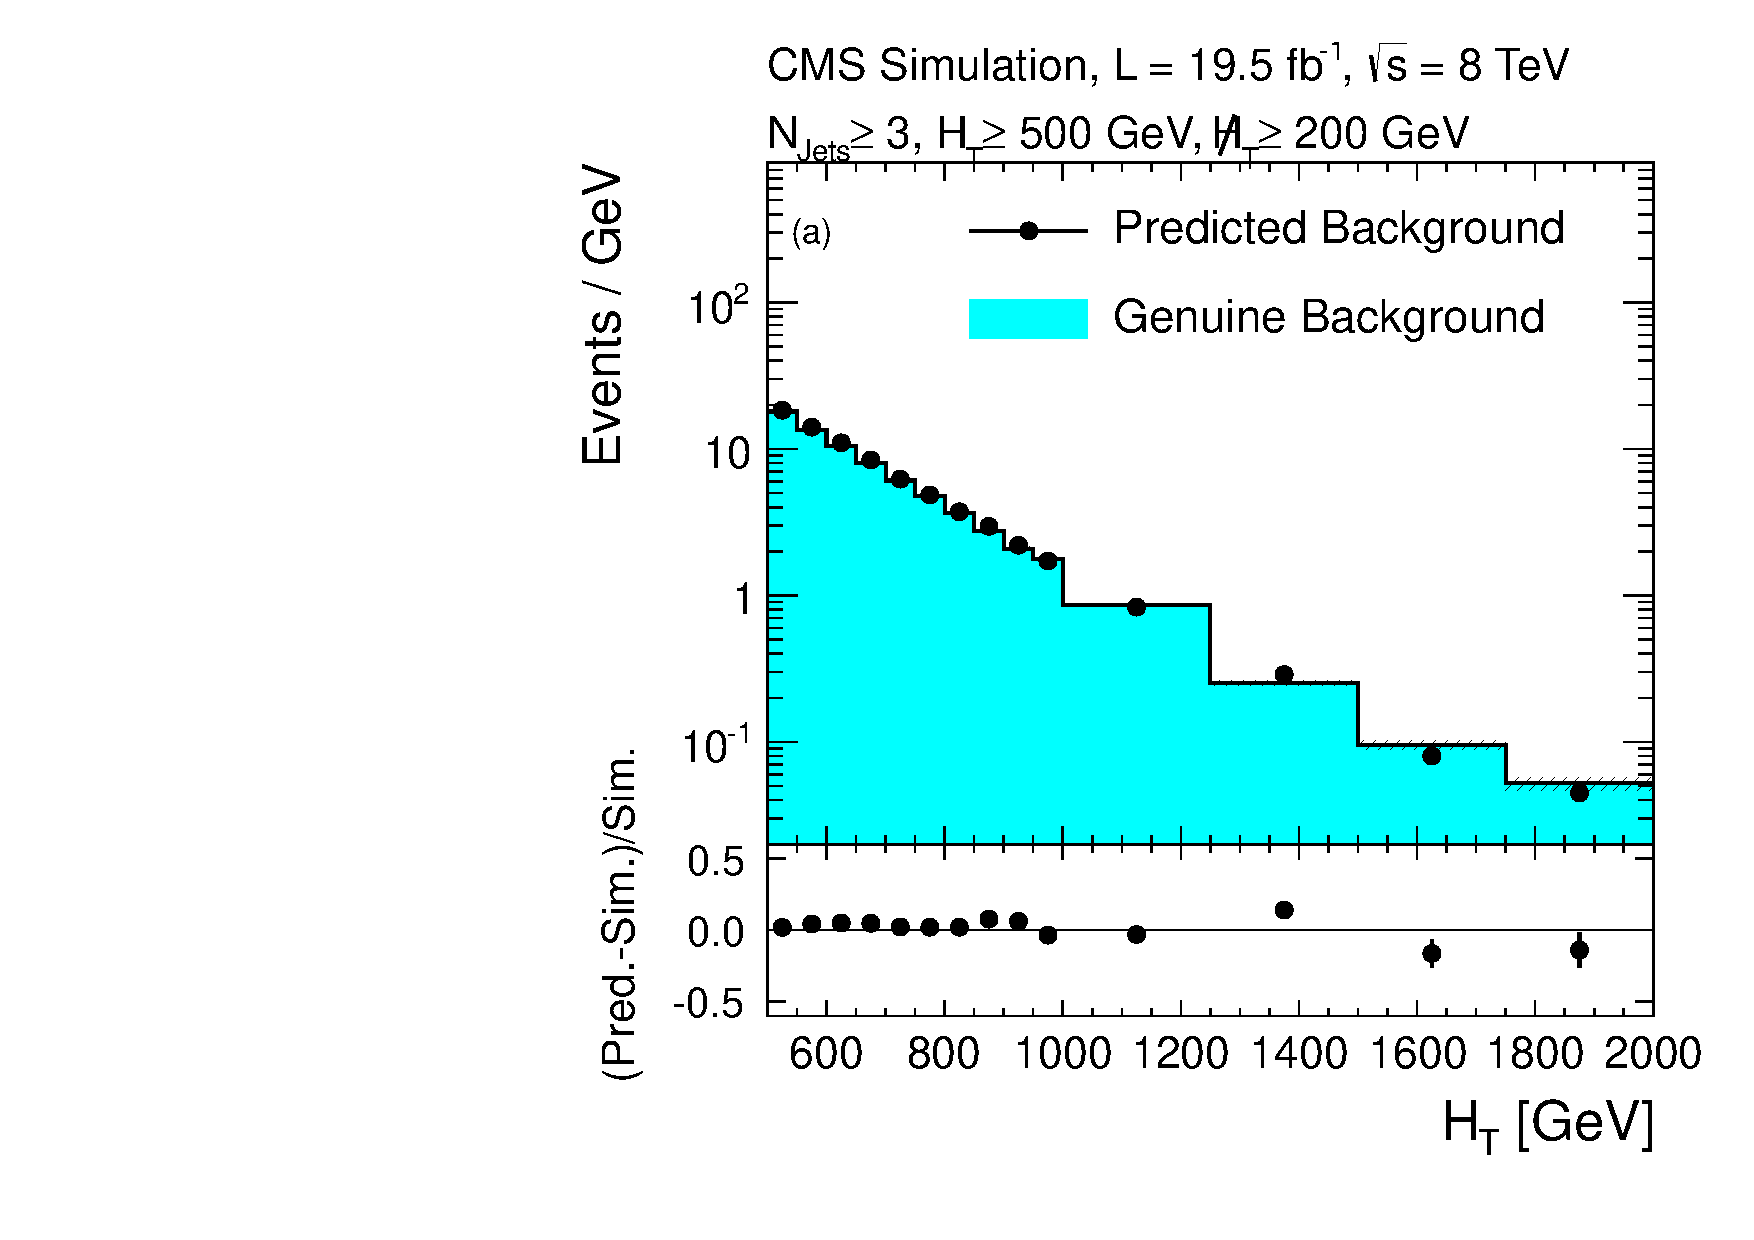
\includegraphics[width=0.4\textwidth]{figures/RA2_TauHad1.pdf} & 
                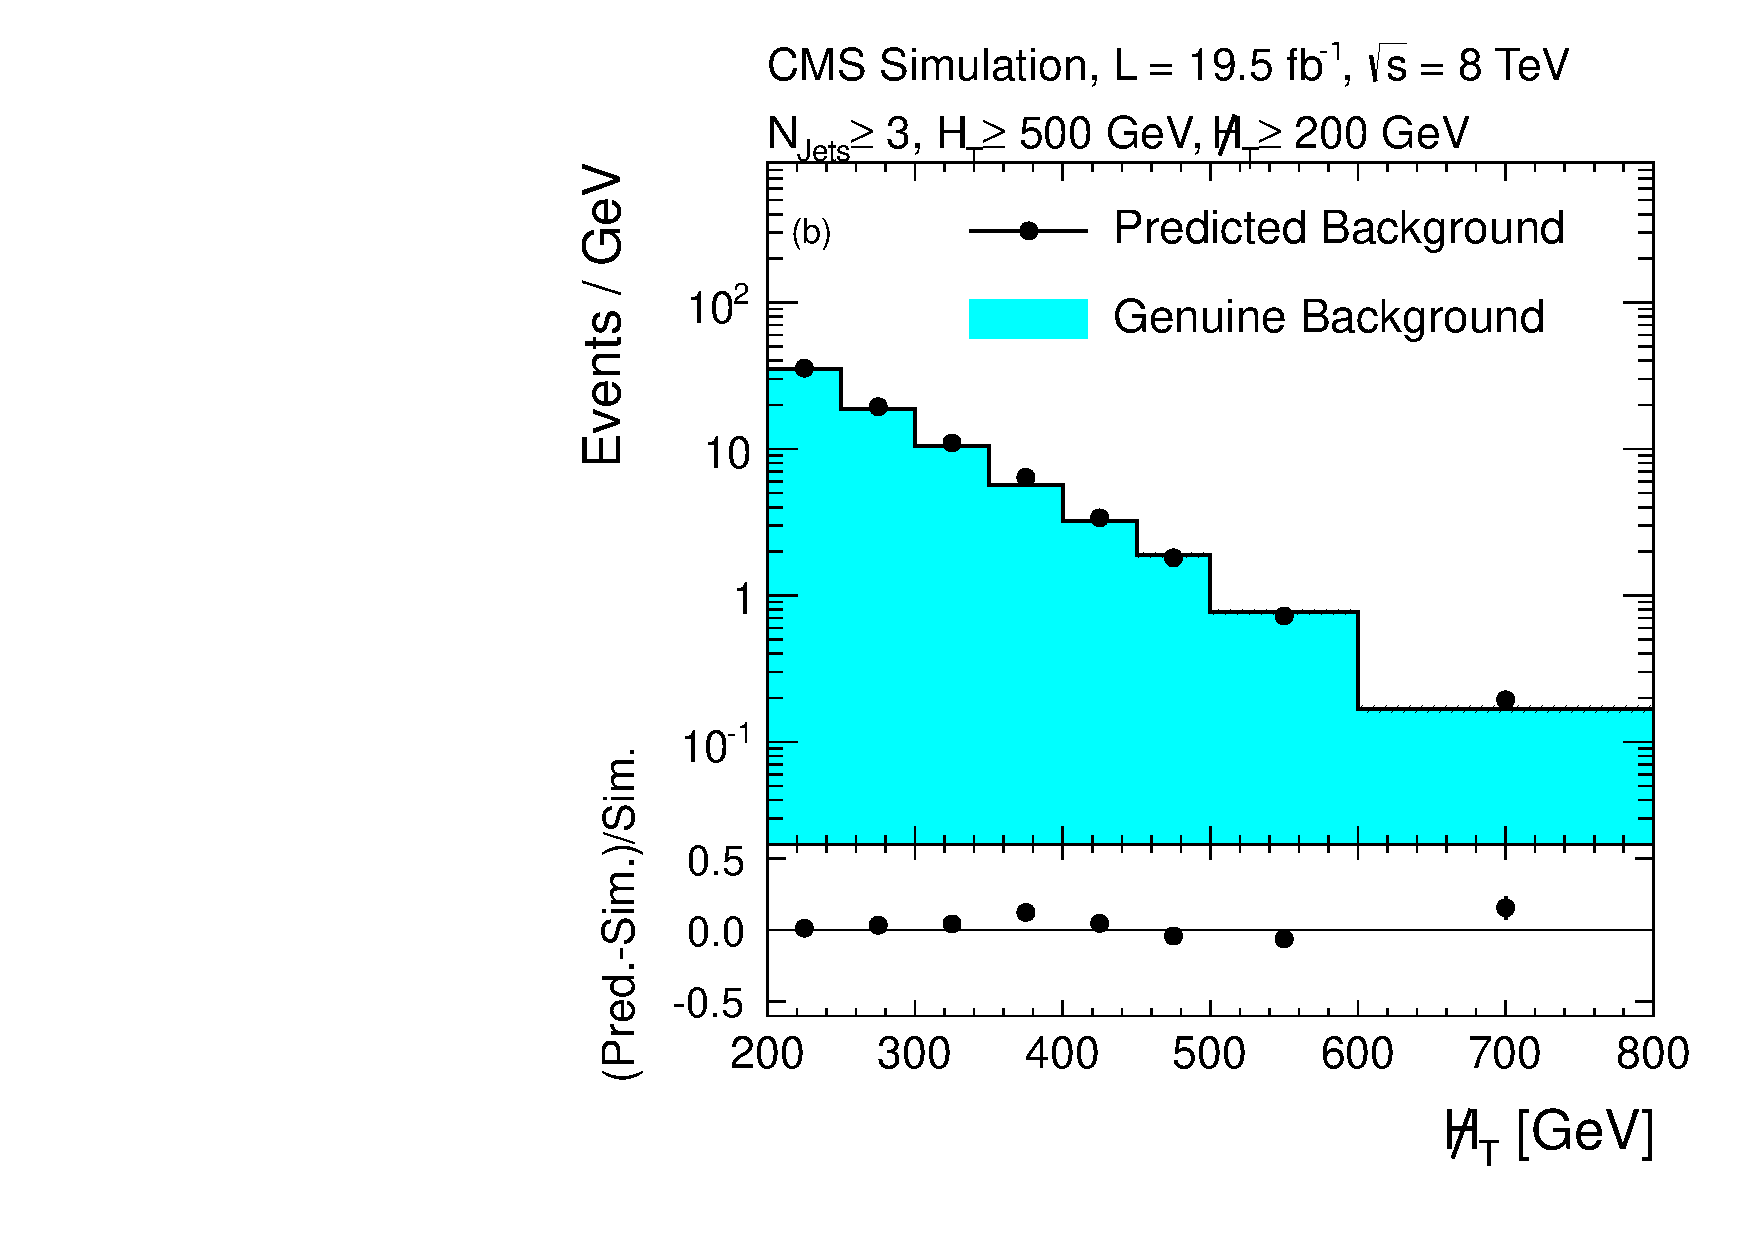
\includegraphics[width=0.4\textwidth]{figures/RA2_TauHad2.pdf} &
                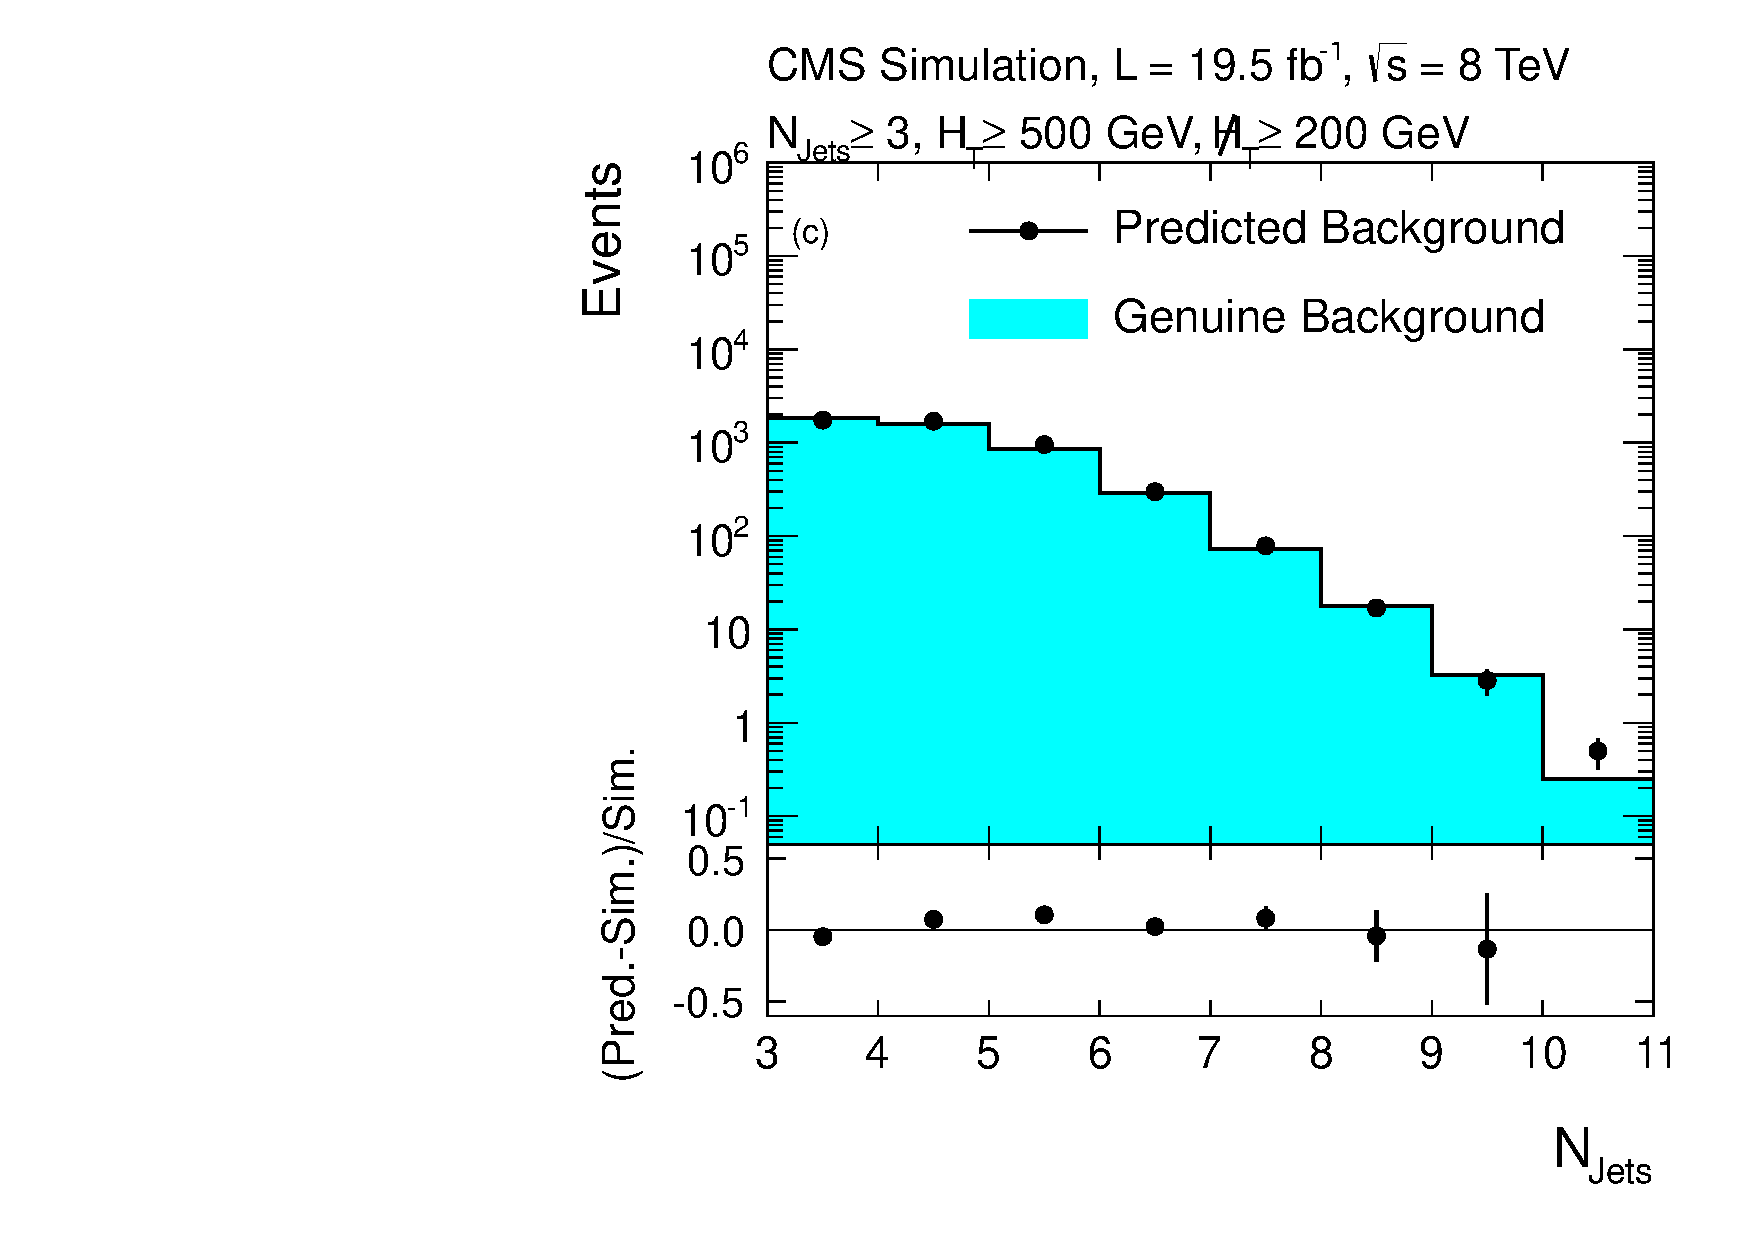
\includegraphics[width=0.4\textwidth]{figures/RA2_TauHad3.pdf}
  \end{tabular}}
  \caption{Predicted (a) HT, (b) MHT, and (c) NJets distributions found from applying the hadronic-tau background evaluation method to simulated $t\bar{t}$ and W+jets events (solid points) in comparison to the genuine $t\bar{t}$ and W+jets background from simulation (shaded curve). Only statistical uncertainties are shown. Taken from~\cite{Chatrchyan:2014lfa}.}
  \label{fig:ra2_tauhad}
\end{figure}

\subsection{Lost-Lepton Background}
\label{subsec:RA2_lostlepton}

\begin{figure}[!h]
  \centering
\makebox[\linewidth]{
  \begin{tabular}{ccc}
                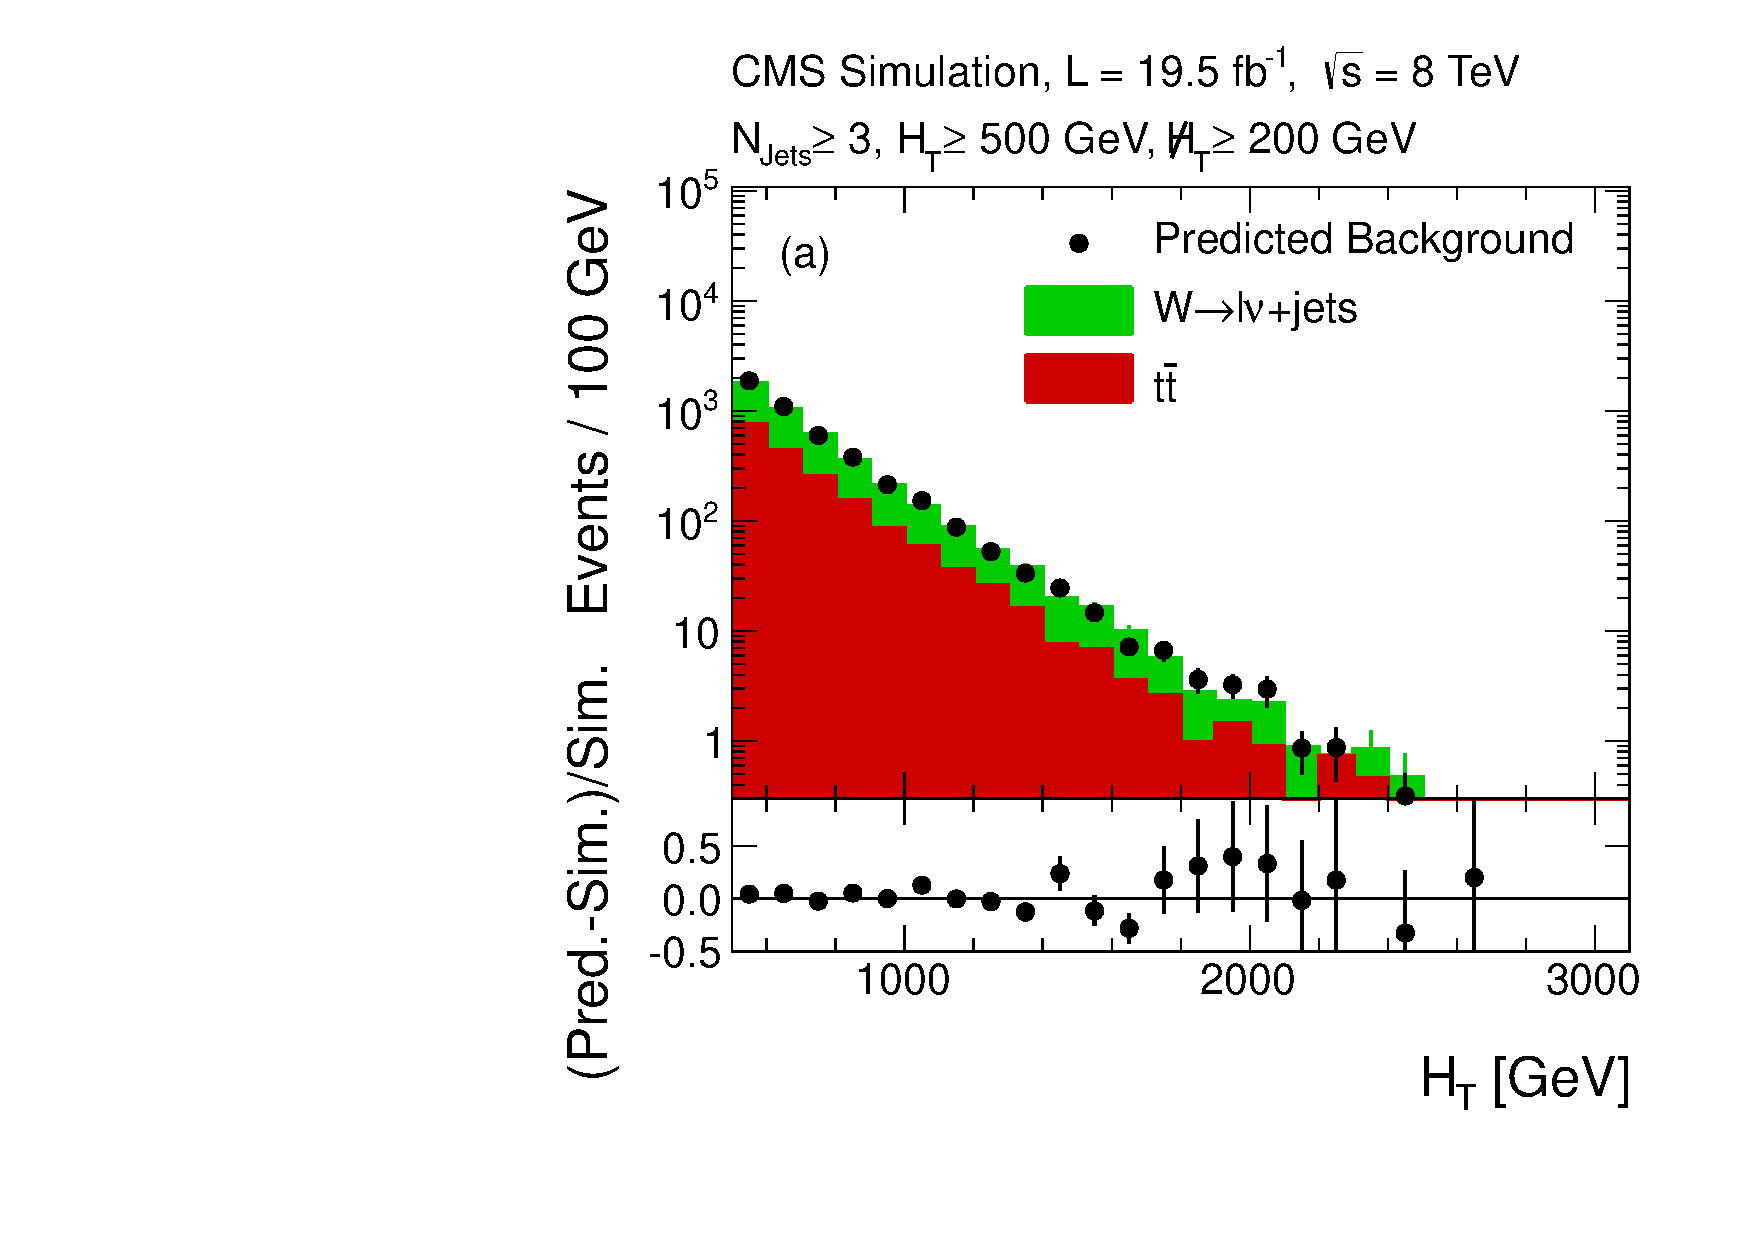
\includegraphics[width=0.4\textwidth]{figures/RA2_LL1.pdf} & 
                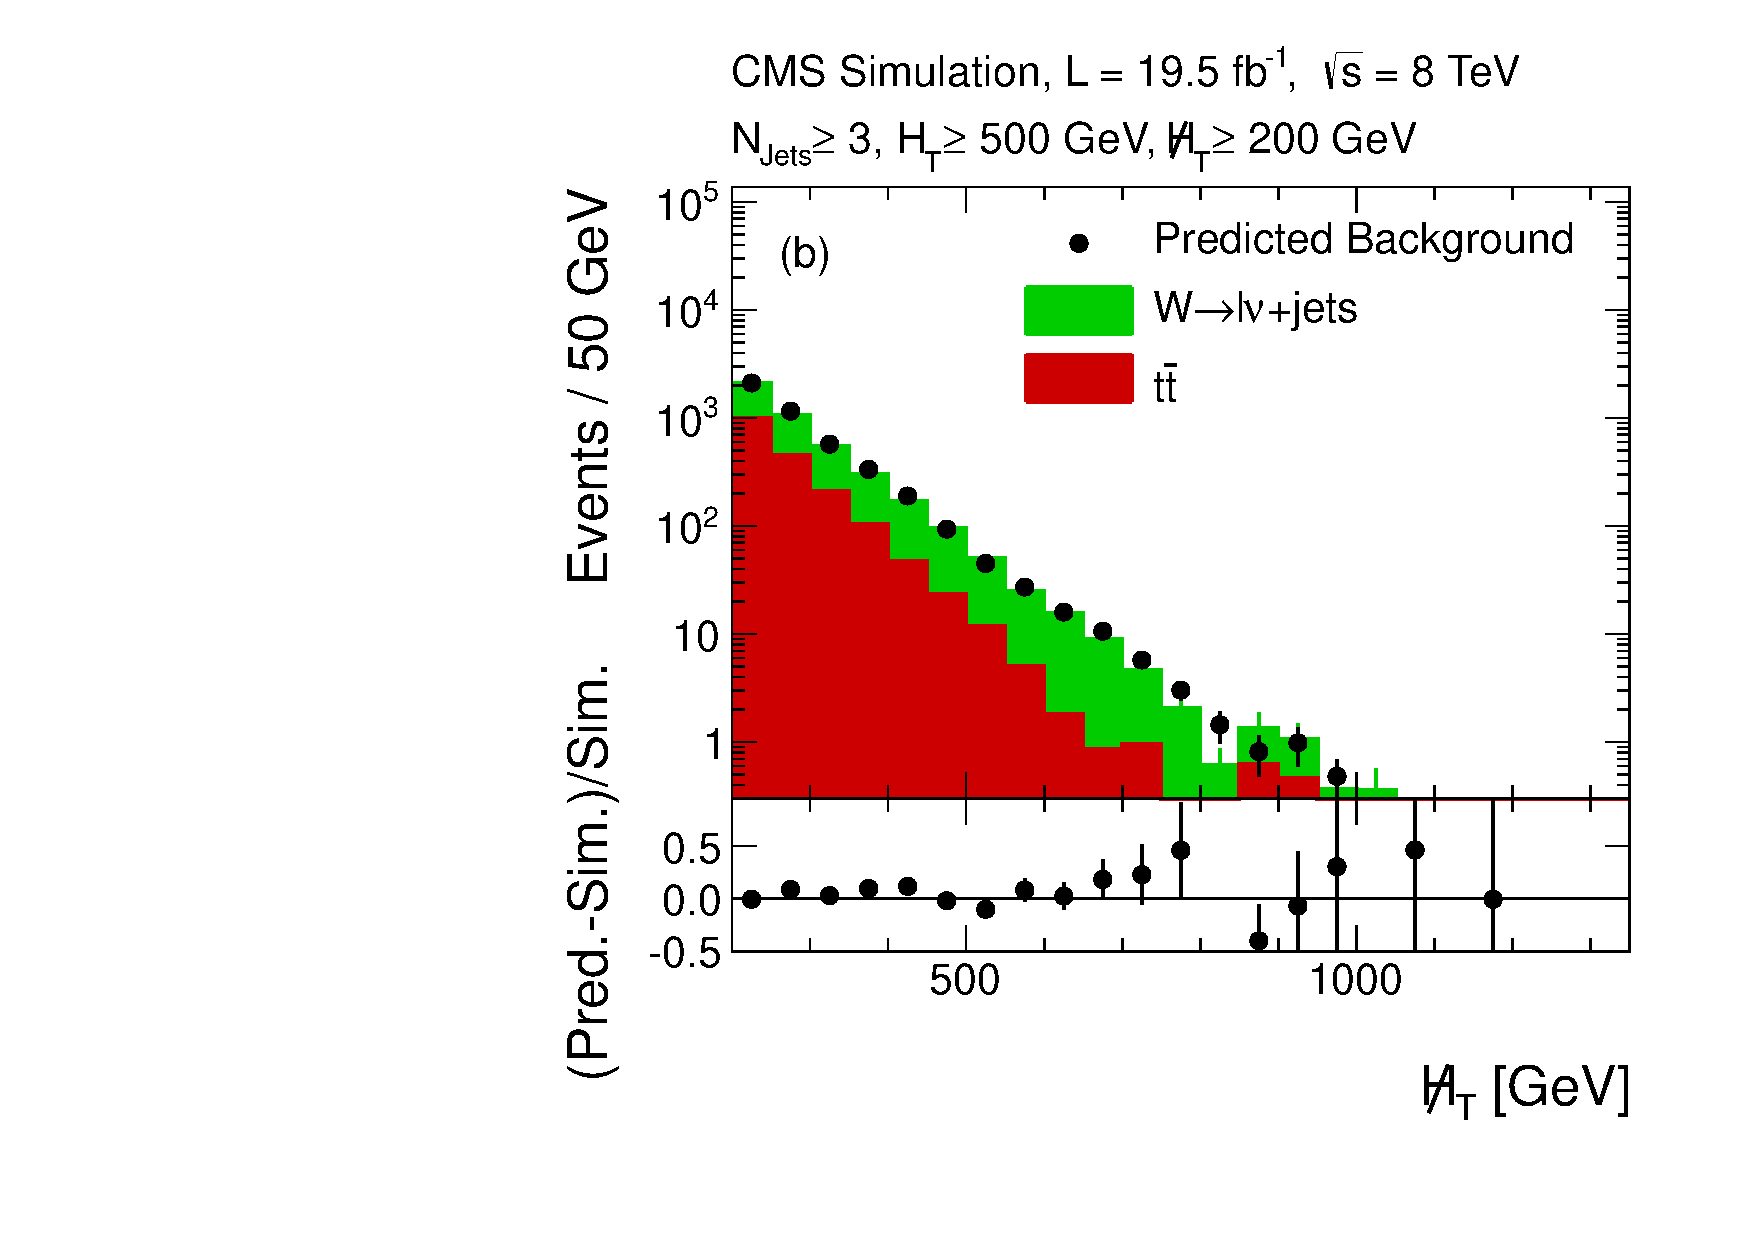
\includegraphics[width=0.4\textwidth]{figures/RA2_LL2.pdf} &
                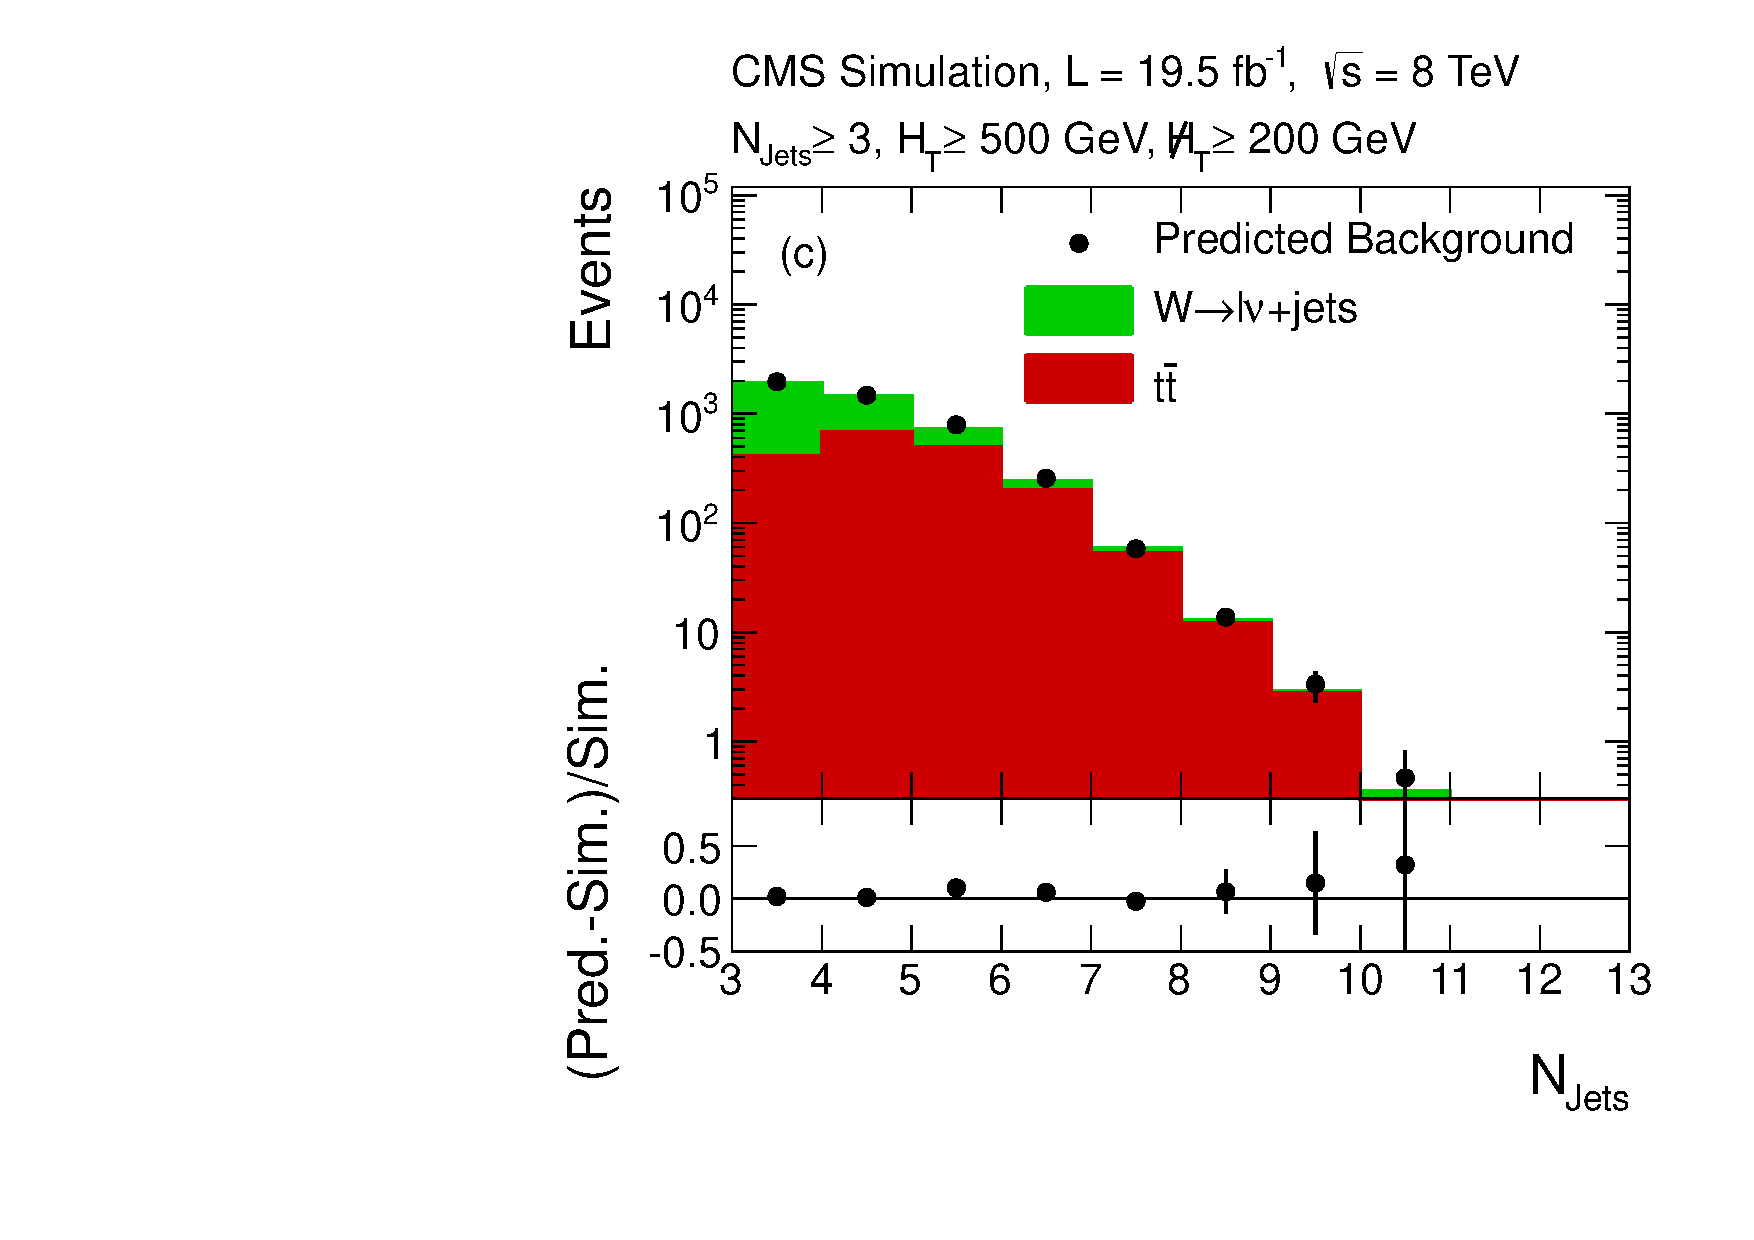
\includegraphics[width=0.4\textwidth]{figures/RA2_LL3.pdf}
  \end{tabular}}
  \caption{Predicted (a) HT, (b) MHT, and (c) NJets distributions found from applying the lost lepton background evaluation method to simulated $t\bar{t}$ and W+jets events (solid points) in comparison to the genuine $t\bar{t}$ and W+jets background from simulation (shaded curves). Only statistical uncertainties are shown. Taken from~\cite{Chatrchyan:2014lfa}.}
  \label{fig:ra2_ll}
\end{figure}

\section{Results and Interpretation}
\label{sec:RA2_results}

\subsection{Comparison to Other Measurements}
\label{subsec:RA2_comp}

\begin{figure}[!tp]
  \centering
  \begin{tabular}{c}
    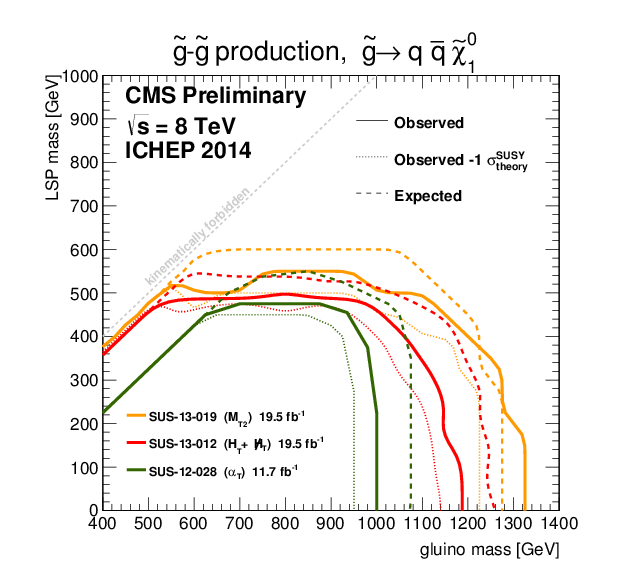
\includegraphics[width=0.9\textwidth]{figures/T1_ICHEP2014_All.png}
  \end{tabular}
  \caption{Comparison of various exclusion limits derived by different CMS analyses for the SMS T1qqqq. Taken from ... (cms susy public results).}
  \label{fig:T1_comp}
\end{figure}

\begin{figure}[!tp]
  \centering
  \begin{tabular}{c}
    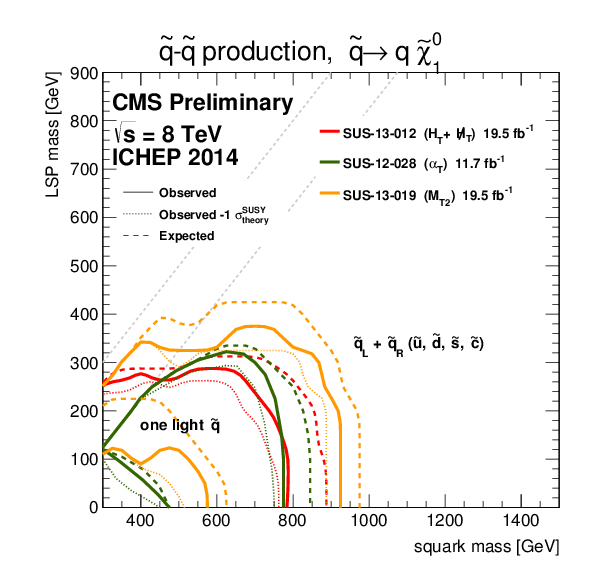
\includegraphics[width=0.9\textwidth]{figures/T2_ICHEP2014.png}
  \end{tabular}
  \caption{Comparison of various exclusion limits derived by different CMS analyses for the SMS T2qq. Taken from ... (cms susy public results).}
  \label{fig:T1_comp}
\end{figure}

\begin{figure}[!tp]
  \centering
  \begin{tabular}{c}
    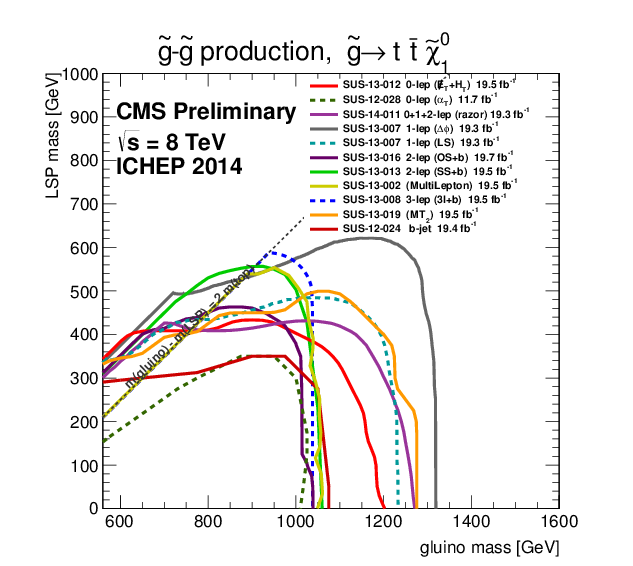
\includegraphics[width=0.9\textwidth]{figures/T1tttt_ICHEP2014_All.png}
  \end{tabular}
  \caption{Comparison of various exclusion limits derived by different CMS analyses for the SMS T1tttt. Taken from ... (cms susy public results).}
  \label{fig:T1_comp}
\end{figure}

\section{Status of natural supersymmetry after LHC Run-I}
\label{sec:susy_status}


